%\documentclass[twocolumn,linenumbers,trackchanges]{tex/aastex631}
\documentclass{aa}
\usepackage{xcolor}
\usepackage{trackchanges}
\usepackage{gensymb}
\usepackage[colorlinks,allcolors=blue]{hyperref}
%%% Beginning of file 'sample631.tex'
%%
%% Modified 2021 March
%%
%% This is a sample manuscript marked up using the
%% AASTeX v6.31 LaTeX 2e macros.
%%
%% AASTeX is now based on Alexey Vikhlinin's emulateapj.cls 
%% (Copyright 2000-2015).  See the classfile for details.

%% AASTeX requires revtex4-1.cls and other external packages such as
%% latexsym, graphicx, amssymb, longtable, and epsf.  Note that as of 
%% Oct 2020, APS now uses revtex4.2e for its journals but remember that 
%% AASTeX v6+ still uses v4.1. All of these external packages should 
%% already be present in the modern TeX distributions but not always.
%% For example, revtex4.1 seems to be missing in the linux version of
%% TexLive 2020. One should be able to get all packages from www.ctan.org.
%% In particular, revtex v4.1 can be found at 
%% https://www.ctan.org/pkg/revtex4-1.

%% The first piece of markup in an AASTeX v6.x document is the \documentclass
%% command. LaTeX will ignore any data that comes before this command. The 
%% documentclass can take an optional argument to modify the output style.
%% The command below calls the preprint style which will produce a tightly 
%% typeset, one-column, single-spaced document.  It is the default and thus
%% does not need to be explicitly stated.
%%
%% using aastex version 6.3
%\documentclass[linenumbers]{aastex631}

%% The default is a single spaced, 10 point font, single spaced article.
%% There are 5 other style options available via an optional argument. They
%% can be invoked like this:
%%
%% \documentclass[arguments]{aastex631}
%% 
%% where the layout options are:
%%
%%  twocolumn   : two text columns, 10 point font, single spaced article.
%%                This is the most compact and represent the final published
%%                derived PDF copy of the accepted manuscript from the publisher
%%  manuscript  : one text column, 12 point font, double spaced article.
%%  preprint    : one text column, 12 point font, single spaced article.  
%%  preprint2   : two text columns, 12 point font, single spaced article.
%%  modern      : a stylish, single text column, 12 point font, article with
%% 		  wider left and right margins. This uses the Daniel
%% 		  Foreman-Mackey and David Hogg design.
%%  RNAAS       : Supresses an abstract. Originally for RNAAS manuscripts 
%%                but now that abstracts are required this is obsolete for
%%                AAS Journals. Authors might need it for other reasons. DO NOT
%%                use \begin{abstract} and \end{abstract} with this style.
%%
%% Note that you can submit to the AAS Journals in any of these 6 styles.
%%
%% There are other optional arguments one can invoke to allow other stylistic
%% actions. The available options are:
%%
%%   astrosymb    : Loads Astrosymb font and define \astrocommands. 
%%   tighten      : Makes baselineskip slightly smaller, only works with 
%%                  the twocolumn substyle.
%%   times        : uses times font instead of the default
%%   linenumbers  : turn on lineno package.
%%   trackchanges : required to see the revision mark up and print its output
%%   longauthor   : Do not use the more compressed footnote style (default) for 
%%                  the author/collaboration/affiliations. Instead print all
%%                  affiliation information after each name. Creates a much 
%%                  longer author list but may be desirable for short 
%%                  author papers.
%% twocolappendix : make 2 column appendix.
%%   anonymous    : Do not show the authors, affiliations and acknowledgments 
%%                  for dual anonymous review.
%%
%% these can be used in any combination, e.g.
%%
%% \documentclass[twocolumn,linenumbers,trackchanges]{aastex631}
%%
%% AASTeX v6.* now includes \hyperref support. While we have built in specific
%% defaults into the classfile you can manually override them with the
%% \hypersetup command. For example,
%%
%% \hypersetup{linkcolor=red,citecolor=green,filecolor=cyan,urlcolor=magenta}
%%
%% will change the color of the internal links to red, the links to the
%% bibliography to green, the file links to cyan, and the external links to
%% magenta. Additional information on \hyperref options can be found here:
%% https://www.tug.org/applications/hyperref/manual.html#x1-40003
%%
%% Note that in v6.3 "bookmarks" has been changed to "true" in hyperref
%% to improve the accessibility of the compiled pdf file.
%%
%% If you want to create your own macros, you can do so
%% using \newcommand. Your macros should appear before
%% the \begin{document} command.
%%
\newcommand{\vdag}{(v)^\dagger}
\newcommand\aastex{AAS\TeX}
\newcommand\latex{La\TeX}

%% Reintroduced the \received and \accepted commands from AASTeX v5.2
\received{\today}
%\revised{April 1, 2021}
%\accepted{\today}

%% Command to document which AAS Journal the manuscript was submitted to.
%% Adds "Submitted to " the argument.
%\submitjournal{PSJ}

%% For manuscript that include authors in collaborations, AASTeX v6.31
%% builds on the \collaboration command to allow greater freedom to 
%% keep the traditional author+affiliation information but only show
%% subsets. The \collaboration command now must appear AFTER the group
%% of authors in the collaboration and it takes TWO arguments. The last
%% is still the collaboration identifier. The text given in this
%% argument is what will be shown in the manuscript. The first argument
%% is the number of author above the \collaboration command to show with
%% the collaboration text. If there are authors that are not part of any
%% collaboration the \nocollaboration command is used. This command takes
%% one argument which is also the number of authors above to show. A
%% dashed line is shown to indicate no collaboration. This example manuscript
%% shows how these commands work to display specific set of authors 
%% on the front page.
%%
%% For manuscript without any need to use \collaboration the 
%% \AuthorCollaborationLimit command from v6.2 can still be used to 
%% show a subset of authors.
%
%\AuthorCollaborationLimit=2
%
%% will only show Schwarz & Muench on the front page of the manuscript
%% (assuming the \collaboration and \nocollaboration commands are
%% commented out).
%%
%% Note that all of the author will be shown in the published article.
%% This feature is meant to be used prior to acceptance to make the
%% front end of a long author article more manageable. Please do not use
%% this functionality for manuscripts with less than 20 authors. Conversely,
%% please do use this when the number of authors exceeds 40.
%%
%% Use \allauthors at the manuscript end to show the full author list.
%% This command should only be used with \AuthorCollaborationLimit is used.

%% The following command can be used to set the latex table counters.  It
%% is needed in this document because it uses a mix of latex tabular and
%% AASTeX deluxetables.  In general it should not be needed.
%\setcounter{table}{1}

%%%%%%%%%%%%%%%%%%%%%%%%%%%%%%%%%%%%%%%%%%%%%%%%%%%%%%%%%%%%%%%%%%%%%%%%%%%%%%%%
%%
%% The following section outlines numerous optional output that
%% can be displayed in the front matter or as running meta-data.
%%
%% If you wish, you may supply running head information, although
%% this information may be modified by the editorial offices.
\shorttitle{AASTeX v6.31 Sample article}
\shortauthors{Schwarz et al.}
%%
%% You can add a light gray and diagonal water-mark to the first page 
%% with this command:
%% \watermark{text}
%% where "text", e.g. DRAFT, is the text to appear.  If the text is 
%% long you can control the water-mark size with:
%% \setwatermarkfontsize{dimension}
%% where dimension is any recognized LaTeX dimension, e.g. pt, in, etc.
%%
%%%%%%%%%%%%%%%%%%%%%%%%%%%%%%%%%%%%%%%%%%%%%%%%%%%%%%%%%%%%%%%%%%%%%%%%%%%%%%%%
\graphicspath{{./}{figures/}}
%% This is the end of the preamble.  Indicate the beginning of the
%% manuscript itself with \begin{document}.

 

\usepackage{graphicx}

\definecolor{cmt}{rgb}{0.5,0.0,0.0}
\definecolor{al}{rgb}{0.6,0.2,0.0}
\definecolor{mk}{rgb}{0.4,0.4,0.0}
\definecolor{no}{rgb}{0,0.0,0.4}
\definecolor{ns}{rgb}{0.4,0.0,0.0}
\definecolor{hr}{rgb}{0.4,0.0,0.0}

\newcommand{\al}[1]{{\color{al}AL: #1}}
\newcommand{\mk}[1]{{\color{mvn}MJK: #1}}
\newcommand{\no}[1]{{\color{corr}NO: #1}}
\newcommand{\ns}[1]{\textsc{\color{al}NS: #1}} 
\newcommand{\hr}[1]{\textbf{\color{ref}HR: #1}} 
\newcommand{\todo}[1]{{\color{cmt}ToDo: #1}}
\newcommand{\cmt}[1]{
{\color{cmt}#1}
}

%\renewcommand{\fig}[1]{Fig.~\ref{#1}} 
\newcommand{\fig}[1]{Fig.~\ref{#1}} 
\newcommand{\Fig}[1]{Figure~\ref{#1}} 
\newcommand{\eq}[1]{Eq.~\ref{#1}} 
\newcommand{\figs}[1]{Figs.~\ref{#1}} 
\newcommand{\tab}[1]{Tab.~\ref{#1}} 
\newcommand{\Tab}[1]{Table~\ref{#1}} 
\newcommand{\sect}[1]{Sec.~\ref{#1}} 
\newcommand{\Sect}[1]{Section~\ref{#1}} 
\newcommand{\secs}[1]{Sections~\ref{#1}} 
\newcommand{\app}[1]{App.~\ref{#1}} 


\newcommand{\kms}{km\,s$^{-1}$}
\newcommand{\ms}{m\,s$^{-1}$}
\newcommand{\grad}{$^\circ$}
\newcommand{\carcsec}{$\mbox{.\hspace{-0.5ex}}^{\prime\prime}$}
\newcommand{\halpha}{H$\alpha$}
\newcommand{\hminus}{H$^-$}
\newcommand{\hei}{He\,\textsc{i}}
\newcommand{\sii}{Si\,\textsc{i}}
\newcommand{\fei}{Fe\,\textsc{i}}
\newcommand{\tii}{Ti\,\textsc{i}}
\newcommand{\cai}{Ca\,\textsc{i}}
\newcommand{\caii}{Ca\,\textsc{ii}}
\newcommand{\caiih}{Ca\,\textsc{ii\,h}}
\newcommand{\coi}{Co\,\textsc{i}}
\newcommand{\helixp}{\textsc{HeLIx$^+$}}
\newcommand{\imax}{{IMaX}}
\newcommand{\sufi}{\textsc{SuFI}}
\newcommand{\sunrise}{\textsc{Sunrise}}
\newcommand{\los}{${\rm LOS}$}
\newcommand{\vlos}{$v_{\rm LOS}$}

\newcommand{\IN}{internetwork}
\newcommand{\inw}{\textsl{INw}}
\newcommand{\nw}{\textsl{Nw}}
\newcommand{\brms}{$B_{\rm RMS}$}

\newcommand{\colfig}[3][1.]{\begin{figure}\centering
    \includegraphics[width=#1\linewidth,clip=TRUE]{#2}
    \caption{#3}
    \label{#2}
\end{figure}}
\newcommand{\colfigtwocol}[3][1.]{\begin{figure*}\centering
    \includegraphics[width=#1\linewidth,clip=TRUE]{#2}
    \caption{#3}
    \label{#2}
\end{figure*}}


\graphicspath{{./figures/}}

\begin{document}
%\title{Quiet-Sun Magnetism Depends on Solar Activity}
\title{Solar-Cycle Variation of quiet-Sun Magnetism and Surface Gravity Oscillation Mode}
%\shorttitle{Quiet-Sun Solar Activity}
\titlerunning{Quiet-Sun Solar Activity}

%\shortauthors{Aalto-f-mode gang.}
%\authorrunning{Olspert et al.}
\authorrunning{Korpi-Lagg et al.}

%\author{N. Olspert\inst{1} \and H. Raichur\inst{2} \and A. Lagg\inst{1,3} \and M. J. K\"apyla\inst{1,4} \and H.-L. Truong\inst{1} \and N. K. Singh\inst{2}}
\author{M. J. Korpi-Lagg\inst{1,4} \and A. Korpi-Lagg\inst{1,3} \and H.-L. Truong\inst{1} \and N. K. Singh\inst{2}}
\institute{Department of Computer Science, Aalto University, PO Box 15400, FI-00076 Aalto, Finland \and
Inter-University Centre for Astronomy and Astrophysics,
 Post Bag 4, Ganeshkhind, Pune 411 007, India \and
Max Planck Institute for Solar System Research, Justus-von-Liebig-Weg 3, D-37077 G\"ottingen, Germany \and
Nordita, KTH Royal Institute of Technology and Stockholm University, 
              Hannes Alfv\'ens v\"ag 12, SE-10691 Stockholm, Sweden
}



\abstract{Bla}{Bla}{Bla}{Bla}{Bla}

%\end{abstract}

%% Keywords should appear after the \end{abstract} command. 
%% The AAS Journals now uses Unified Astronomy Thesaurus concepts:
%% https://astrothesaurus.org
%% You will be asked to selected these concepts during the submission process
%% but this old "keyword" functionality is maintained in case authors want
%% to include these concepts in their preprints.
\keywords{Sun}

\maketitle

\section{Introduction} \label{sec:intro}

\begin{itemize}
\item quiet Sun magnetism is weak. Measurement requires high sensitivity, high spatial resolution, otherwise signal cancellation. Variations in quiet Sun magnetism are even tougher to detect. Require long-term stability, constant conditions, HMI offers this, now 1 solar cycle in orbit. 
\item what is the quiet Sun? simple: No AR. 98\% of the solar surface are in this state. But even the quiet regions are structured: network / internetwork. 
\item what is expected to vary with solar cycle? network, IN, both, or nothing? A few words about the expectations.
\item argue why taking into account network is important: the IN flux is advected towards the network boundaries. A cycle variation of the IN flux therefore should be reflected in a variation of the network flux. Network accumulates IN flux and therefore acts as a memory of what happened in the IN. Helps to overcome detection of the weak IN fields (difficult enough), even more difficult to study variations of these weak fields.
\item HMI: compared to Hinode / ground based / Sunrise: not the most sensitive instrument to B. But: Stability allows averaging. 8 hr time and spatial averaging allows to boost S/N ratio (can we give a number here?)

\end{itemize}

\cite[]{2019LRSP...16....1B}
Luis Talk PHI meeting: 38\% of the flux emerging in the IN makes it to the network. Network flux is constant, the IN flux to the network accumulates quickly to network flux.

\cite[]{2015ApJ...806..174J}

\cite[]{2013A&A...555A..33B}

\cite[]{2021arXiv210508657F}

\cite[]{2021arXiv210514533R}

\cite[]{ballot2021changes}


\section{Observations}

Our analysis is based on data from the Helioseismic Magnetograph and Imager \cite[HMI,][]{2012SoPh..275..207S,2012SoPh..275..229S} on board the Solar Dynamics Observatory \cite[SDO,][]{2012SoPh..275....3P}. We use two standard data products: (i) full-disk line-of-sight (LOS) magnetograms, computed every 720\,s by comining filtergrams obtained over a time interval of 1260\,s (\texttt{hmi.M\_720s}), and (ii) full-disk LOS dopplergrams, computed every 45\,s from six positions across the nominal 6173.3\,\AA{} spectral line (\texttt{hmi.V\_45s}). We processed the two data sets in a semi-automatic pipeline (see \fig{pipeline}), optimized for obtaining reliable information abount the magnetic field in the quiet Sun regions and for a robust computation of the $f$-mode power from the dopplergrams. The left tree in \fig{pipeline} describes the pipeline used for the magnetograms, the right tree for the dopplergrams.

\colfig{pipeline}{Data pipeline}

\subsection{Magnetograms}

The first data product, full-disk line-of-sight (LOS) magnetograms, provides a direct measurement of the variability of the quiet-sun magnetism during a solar cycle. To enhance the signal-to-noise ratio in the LOS magnetograms we performed a newly developed algorithm for spatial and temporal averaging: The full-disk HMI magnetograms starting from 27-Apr-2010 and ending at \todo{01-Oct-2021} were downloaded from the Joint Science Operation Center (JSOC) hosted at Stanford University (http://jsoc.stanford.edu) to a temporary storage (see \fig{pipeline}, 'mahti storage') and tracked at full spatial resolution for 8 hours to compensate for the solar rotation ('full disk tracking').
\al{@Nigul: Can you explain the differntial rotation model used?}. 
The step between tracked sequences was 4 hours, so that a total of 6 tracked sequences were gathered per one day, resulting in more than $24\,000$ tracked sequences.

From each tracked sequence, we extracted two data products by dividing the visible solar disk  between latitudes and longitudes from $-80\degree$ to +$80\degree$ into (i) $64\times 64$  overlapping patches of $15\degree$ (in solar latitude and longitude)  and (ii) $180\times 180$ patches of $1\degree$.
Every of these patches therefore contains a space-time cube of LOS magnetograms at full spatial resolution at a 12-minute cadence, allowing to compute the statistical properties (mean, standard deviation, skewness, kurtosis) of the following parameters: $<B>$ -- mean of the magnetic field strength, $<|B|>$ -- mean of the absolute value of the magnetic field strength, and $\sqrt{<B^2>}}$ -- root mean square of the magnetic field strength (\brms{}). The $15\degree$ patches (i) are large enough to cover several supergranulation cells containing network and \IN{} fields \cite[]{2010LRSP....7....2R} with a typical size of 30--35\,Mm (we refer to them as \nw{} cubes), and the $1\degree$ patches (ii) are small enough that some of them lie completely in the \IN{} (\inw{} cubes). 
The statistics for each patch were stored as data products (see also \fig{pipeline}) including the information about latitudinal and longitudinal position as well as the Carrington longitude for network and \IN{}. We refer to these maps as the \nw{} and the \inw{} statistical maps.

 
% \begin{itemize}
% 	\item $\mu_B$ -- Mean of the magnetic field strength
% 	\item $\sigma_B$ -- Standard deviation of the magnetic field strength
% 	\item ${\rm skew}_B$ -- Skewness of the magnetic field strength
% 	\item ${\rm kurt}_B$ -- Kurtosis of the magnetic field strength
% 	\item $\mu_{|B|}$ -- Mean of the absolute value of the magnetic field strength
%     \item $\sigma_{|B|}$ --Standard deviation of the absolute value of the magnetic field strength
%     \item ${\rm skew}_{|B|}$ -- Skewness of the absolute value of the magnetic field strength
%     \item ${\rm kurt}_{|B|}$ --Kurtosis of the absolute value of the magnetic field strength
% 	\item \brms{} -- Root mean square of the magnetic field strength
%     \item $\sqrt{\sigma:{B^2}}$ -- Root mean square of the standard deviation of the magnetic field strength
%     \item $\sqrt{{\rm skew}_{B^2}}$ -- Root mean square of the skewness of the magnetic field strength
%     \item $\sqrt{{\rm kurt}_{B^2}}$ -- Root mean square of the kurtosis of the magnetic field strength
% \end{itemize}

\subsection{Quiet region selection\label{quietregion}}

From the parameters computed from the cubes the root mean square of the magnetic field strength (\brms{}) turned out to be the best tracer for determining the magnetic activity level. It could clearly distinguish between $15\degree$ patches containing active regions, plage, enhanced network and quiet network. Also, it depicted very well the low-field \IN{} regions.

The analysis of the solar-cycle variation of the quiet-sun magnetism required a careful selection of the most quiet regions, defined as being free of enhanced solar activity. We therefore searched for the minimum value of \brms{} in both, the \nw{} and the \inw{} statistical maps, on a latitudinal grid with a $10\degree$ spacing fulfilling the following additional criteria:
\begin{enumerate}[(i)]
	\item\label{c1} the most quiet pixel must be within $\pm10\degree$ around the central meridian,
	\item\label{c2}  this pixel must belong to the 3\% most quiet pixels of the month,
	\item\label{c3}  this pixel must be the most quiet pixel within a 4-day interval.
\end{enumerate}

Criterion (\ref{c1}) was chosen to get the strongest magnetic field signal along the central meridian. (\ref{c2}) guarantees an equal distribution of quiet pixels over the 11-year period of available HMI measurements, and (\ref{c3}) ensures that the quiet pixels for the 1-month period do not originate from the same supergranular structure, since the dynamical evolution time of the supergranulation lies between 24 and 48\,h \cite[]{2010LRSP....7....2R}. The result of this selection were two time series of the \brms{} for the most quiet patches in the network and the \IN{} regions. Note that the this selection also efficiently removes the 24\,h modulation present in the HMI magnetograms.

\subsection{Correction for HMI sensitivity change\label{sensicorr}}

The 11-year temporal evolution of \inw{} time series{the \brms{}} value revealed clearly a change in the HMI observing mode, performed on 13-Apr-2016. On this day, HMI switched to a more efficient observing mode \cite[see][]{2018SoPh..293...45H,2014SoPh..289.3483H,2016SoPh..291.1887C}. By combining both HMI cameras to determine the vector-field observables the cadence for full-disk magnetograms could be reduced from 135\,s (observational mode MOD-C) to 90\,s (MOD-L). This reduced the noise level for Stokes $V$ measurements by 17\%, resulting in a decrease of the noise level in the \los{} magnetograms by 5\%.

For the long-term study presented in this paper, we need to correct for this sensitivity change. A very accurate correction method can be derived from the \inw{} time series: since it contains only the most quiet pixels over a certain latitude region and time, the sensitivity change results in a step function. The value of the step was determined by fitting a polynomial to the \brms{} values determined from the \inw{} time series plus a Heaviside step function, centered at the date of the mode change. We used the Bayesian information criterion \cite[BIC,][]{Stoica2004} to determine the degree of the polynomial, which lies between 1 and 6 for the various latitudes. We want to note that the retrieved amplitude of the Heaviside step function is only weakly dependant on the degree of the polynomial. This fitting is exemplified in \fig{fit-offset} for the solar latitude 0$^\circ$, where the minimum value for the BIC was reached for a fit with a polynomial of degree 4. The so determined amplitude of the Heaviside step function is added to the data points after 13-Apr-2016 for all data presented in this paper.



\colfig{fit-offset}{Determination of the correction for the HMI sensitivity change: the observing mode change on April 13 2016 causes a discontinuity in the level of \brms{} values of the \IN{} data. The original data are displayed in with the dark red and black dots, the corrected data with the light red dots. The dashed line indicates the polynomial fit of degree 4 used to obtain the offset.}




% \cmt{
% Key issue: 
% How to obtain the most reliable HMI data product telling us about the variability of the quiet Sun magnetism during a solar cycle? Idea: combine spatial and temporal averaging, and analyze the statistics in space-time cubes to determine the level of quietness as a function of latitude. This requires the magnetic field information coming from specro-polarimetry. 

% But first the boring stuff: How to obtain a clean, 11-year long data set:

% About the long term trend: The jump in the data happened on 13 April 2016 (search for this date in \cite{2018SoPh..293...45H}). There it states:
% \begin{itemize}
% \item Standard HMI observations were initially obtained with a framelist called Mod-C that
% repeated every 135 seconds. Mod-L, a 90-second FTS, replaced Mod-C on 13 April 2016.
% The two versions of Mod-C have FTS ID 1001 or 1021; the Mod-L HFTSACID is 1022.
% Some calibration framelists changed when the standard sequences changed.
% \item Since 13 April
% 2016, filtergrams from the two cameras have been combined to compute the vector magnetic
% field \cite[]{2014SoPh..289.3483H,2016SoPh..291.1887C}
% \item On 13 April 2016, after the prime mission ended, HMI switched to
% a faster sequence, FTS ID 1022, also known as Mod-L. The Mod-L sequence requires that
% images from both cameras be combined to determine the vector-field observables. 
% \end{itemize}
% Mod-L description here: http://hmi.stanford.edu/hminuggets/?p=1596: \textsl{
% Mod-L provides all of the filtergrams necessary to compute the Stokes parameters [I, Q, U, V] in 90 seconds, instead of the 135 seconds required for Mod-C. Thus Mod-L increases the maximum temporal resolution for measuring full Stokes parameters. At the same time, it decreases the noise because twice as many filtergrams are available. The 45s data products from the front camera are also improved; since there is no longer a 135s period in the instrument configuration, the corresponding peak in the Doppler power spectrum is now gone. The new 90s period is at the Nyquist frequency of the 45s-cadence Doppler data. The Stokes measurement is normally averaged over time (nominally 720 seconds) to derive [I, Q, U, V], and we now combine three times as many CP and 1.5 times as many LP measurements. Table 1 compares the Mod-C and Mod-L observations.}
% }



\subsection{Dopplergrams}

The second data product used in this paper are the \los{} velocity maps. The goal is to compute the power of the surface gravity mode, the so-called $f$-mode power, as an independent measure to quantify the solar cycle variation.

The dopplergram data is hosted in the German Data Center for SDO (GDC-SDO) on a server at the Max Planck Institute for Solar System Research (MPS Göttingen, Germany) whereas the analysis is executed in the CSC supercomputing environment (Aalto, Finland). We have utilized  a function-as-a-service client based on funcX \cite[]{chard20funcx} for accessing the required data in the database server. We have developed functions based on funcX API and deployed the functions in the MPS environment. These functions leverage the mtrack\footnote{\url{http://hmi.stanford.edu/teams/rings/modules/mtrack/v25.html}} command to prepare the dopplergram cubes within the GDC-SDO environment and subsequently transfer them to the CSC environment. The coordinates of the selected quiet-sun regions were sent to the funcX service, which invokes suitable functions to automate the data retrieval and movement.
%{the using remote function call service funcX \cite{chard20funcx} to MPS server where the dopplergram database is located. Next, using mtrack command the tracked dopplergram cubes were retrieved and sent back to CSC supercomputing environment.}

\todo{details of the tracking: Central coordinate from quiet region selection, Harsha's parameters. $300\times 300$ pixels, 8 hrs ... }

\subsection{Computation of the $f$-mode power}

In the CSC environment, subsequent processing involved calculating the 3d power spectra for each dopplergram cube and averaging the spectra azimuthally in $k_x, k_y$ plane for each constant $\omega$ (See \fig{ring_diagram}). Such averaging significantly reduced the noise level leading to smooth one dimensional $k-\omega$ spectra. Such averaging is justified for the quiet-sun spectra, as the ring diagrams are radially symmetrical w.r.t. $\omega$ axis. From the obtained spectra $f$-mode was easily separable from the rest of the modes and integration done over $k$ and $\omega$, to obtain full power of the $f$-mode. The integration range was chosen between $\omega$ values starting from 14.45 and ending at 29.03, where the significant part of the $f$-mode power resides. After completing described steps we had collected total of \todo{18327} $f$-mode powers for patches close to central meridian over all latitudes covering the full solar cycle.

\begin{figure}\centering
	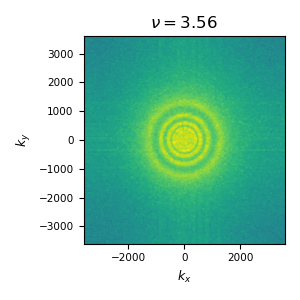
\includegraphics[width=1.0\linewidth,trim={0cm 0.4cm 0cm 0.3cm},clip=TRUE]{ring_diagram}\\
	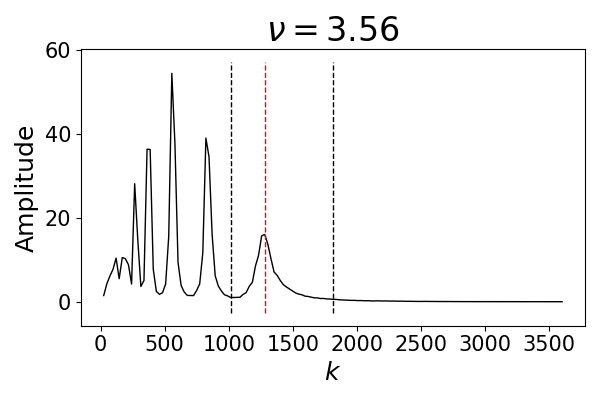
\includegraphics[width=1.0\linewidth,trim={0cm 0cm 0cm 1cm},clip=TRUE]{az_avg_spec}
	\caption{Top: example of quiet-sun ring diagram at $\nu=3.56$. Bottom: spectrum obtained by azimuthally averaging the ring diagram. The red vertical line marks the position of the maximum of the $f$-mode and the black vertical lines the range of integration.}
	\label{ring_diagram}
\end{figure}

\subsubsection*{Orbital correction of the $f$-mode power}

%AL We have to be consistent. Do we call it f-mode power, strength or area?
Since the $f$-mode power is computed from the \los{} dopplergrams, its value depends strongly on the viewing geometry. This dependence,  roughly following the cosine of the solar latitude for data taken at the central meridian, is additionally modulated by the orbital motion of the Earth around the Sun, which changes the viewing angle at any given solar latitude by $\approx\pm7^\circ$ during one year. We compensated for this periodic variation by fitting the parameters ($x_0(\lambda), ..., x_3(\lambda)$) of the following function to all observations of a given latitude $\lambda$:
\begin{equation}
\label{eq:orbitcorr}
A_{\mbox{corr}}(\lambda) = x_0(\lambda) (  2 ( (1+\cos(\alpha+x_1(\lambda)))/2)^{x_3(\lambda)}-1   )+ x_2(\lambda),
\end{equation}
with $\alpha$ being the phase angle of the Earth defined as the cotangens computed from the $x,y$ barycentric position of the Earth.
This correction $A_{\mbox{corr}}(\lambda)$ is then subtracted from the computed $f$-mode power, which efficiently removes any yearly variation. 



\todo{Mention also the focus change in 2018-10-16, leading to a change in the \los{} maps.} 

\section{Results}

After applying the selection criteria described in \sect{quietregion} and the subsequent correction for the HMIS sensitivity change (\sect{sensicorr}) we obtain the dependency of the \brms{} values of the most quiet region at the central longitude as a function of heliographic latitude and time. \fig{Brms-lat00-percentile} presents the \brms{} values from May 2010 until October 2021 for the heliographic latitude $\lambda = 0\degree$. The individual data points (red dots) are computed over an area of 15$^\circ$ in latitude and longitude and over a time of 8 hours. At disk center, this corresponds to an area of $\approx 180 \times 180$\,Mm$^2$, and therefore contains 30--40 supergranular cells. The \brms{} value therfore contans network and \IN{} fields.

\fig{Brms-lat00-percentile} clearly indicates the solar cycle dependence of the quiet-sun magnetic fields, consisting of network and \IN{}. The \brms{} values peak in the second half of 2014, close to the declared maximum od solar cycle \#24 (April 2014, \todo{REF!}. The variation is statistically significant, as indicated by the the mode and the 97\% percentiles, computed by fitting a log-normal distribution over a 1-year sliding window.

A similar plot is presented in \fig{Brms-lat00-percentile-IN}, but now the \brms{} value was computed only for a $1\degree$ window in latitude and longitude, correspondinf to an area of only $12\times 12$\,Mm$^2$ at disk center. The quiet-region selection criteria (\sect{quietregion}) guarantees, that this patch lies fully within the \IN{}, and is not `contaminated' by network fields. Clearly, there is no dependence of \brms{} with solar cycle detectable. The slight increase over the 11-year period might be an effect of the aging of the HMI instrument and the resulting decrease in the sensitivity for magnetic field measurements.

\colfig{Brms-lat00-percentile}{\brms{} determined from the most quiet patches from 2010 to 2021 at disk center. The patches of 15$^\circ$ size in longitude and latitude contain network and \IN{} fields. The solid red lines display the 97\% percentile level, the dashed, gray line the mode of a log-normal fit to yearly-binned data moved in a sliding window of 100 days length.}

\colfig{Brms-lat00-percentile-IN}{Same as \fig{Brms-lat00-percentile}, but for \brms{} determined from patch size of only of 1$^\circ$ in longitude and latitude, corresponding to \IN{} patches. }


\subsection{Butterfly}

Definitions:\\
$\lambda$ = latitude, $t$=time, \\
$N_t$ = number of bins in time \\
$N_\lambda$ = number of bins in latitude, \\
$n_t$ = total number of time points at a certain latitude, \\
$N_P$ = number of $f$-mode measurements in a patch, \\
$\overline{X}$ indicates average over full time span, \\
$\left< X \right>$ indicates an average in a selected bin, \\
%AL: The <> would remove the necessity for the subscript _P, 
% which meant exactly the same
% I removed all the _P and replaced it by <>
$f(\lambda,t)$ = $f$-mode strength \\
%AL removed _P
%$\left<f_P\right>=1/N_P \sum_{N_P} f (\lambda,t)$ = mean $f$-mode strength 
$\left< f \right>=1/N_P \sum_{N_P} f (\lambda,t)$ = mean $f$-mode strength calculated in patches of $N_t$ and $N_\lambda$ \\
$\overline{f}(\lambda) = 1/n_t \sum_t f(\lambda,t)$ = temporal mean of the $f$-mode strength, \\
%MJK This is what is plotted in the butterfly, and should appear in title/caption.
%MJK It is further binned for plotting, the explanation of which is still missing, but this should not be here, but in the figure caption.
$f'=f-\overline{f}$ is the fluctuation around the temporal mean, i.e. the solar cycle dependence of the $f$-mode.\\
%AL: In the butterfly we plot the binned f'. It is computed like this:
$\left< f' \right> = \left< f - \overline{f} \right> $ is the same as $f'$, but computed in $N_\lambda \times N_P$ bins. This is the quantity we show in the left panel of \fig{butterfly_lat}.
%MJK Added
We assume that the solar cycle variation is a sinusoidal function, the amplitude of which can be approximated as 
%AL Would it be more correct if we also use <> around the quantity f'_A?
$f'_{\rm A} (\lambda) = 
\sqrt{2} \sqrt{\left<{f'^2}\right>}$. 
The average over the bin is necessary to remove the noise from the estimate.
%AL added
This quantity $f'_{\rm A} (\lambda)$ is plotted as the orange shaded area in the right panel of \fig{butterfly_lat}.

One measure of the noise contained in the $f$-mode strength is the standard deviation of the fluctuations
around the signal. This is calculated in each bin as
\begin{equation}
\sigma= \sqrt{\frac{1}{N_P}\sum_{\mbox{patch}} ( f(\lambda,t)
- \left<f_P\right>)^2}.
\end{equation}
From this we form the average error at each latitude by taking an average over time and denote as $\overline{\sigma}$. 
%AL added
This quantity is plotted as the error bar in the right panel of \fig{butterfly_lat}.

%NO Adding some words how we verified significance
As the average error described above does not necessarily prove that the patterns seen in the left panel of \fig{butterfly_lat} are statistically significant, we did more detailed analysis and estimated the significance of $\left< f' \right>$ for each patch separately. The following test was made: For all quiet-sun patches we computed the power of noise in the azimuthally averaged spectra similarly as for $f$-modes. We assumed that noise level is independent of $k$ and selected the region towards higher $k$ values, where the $f$-mode is already decayed. Then we calculated fluctuations in the noise power $\left< f'_{\rm noise} \right>$ in an identical manner as for $\left< f' \right>$.
The analysis showed that for all patches $\left< f'_{\rm noise} \right>$ was an order of magnitude weaker than the corresponding $\left< f' \right>$.

%AL BEGIN unnecessary stuff
\color{cyan}
\subsection*{All the stuff below this line not needed !!!}
Error definitions:\\
$\lambda$ = latitude, $t$=time, \\
$N_t$ = number of bins (time), \\
$N_\lambda$ = number of bins (latitude), \\
$N_P$ = number of $f$-mode measurements in a patch, \\
$\overline{X}$ indicates average over time, \\
$f(\lambda,t)$ = $f$-mode strength (unbinned)\\
$f_P(\lambda,t)$ = $f$-mode strength in latitude / time bins (patches)\\
$\overline{f}(\lambda) = 1/N_t \sum_t f(\lambda,t)$ = temporal mean of the $f$-mode strength (unbinned)\\ 
$f'=f-\overline{f}$ is the fluctuation around the temporal mean, i.e. the solar cycle dependence of the $f$-mode (unbinned)\\
$\overline{f_P}(\lambda) = 1/N_t \sum_t f_P(\lambda,t)$ = temporal mean of 
$f$-mode strength (in lat / time bins), \\
$f'_P=f_P-\overline{f_P}$ is, correspondingly, the binned fluctuation\\

%AL added this
The following 4 definitions represent what is plotted in \fig{butterfly_lat_old}:
\begin{itemize}
\item sdev(cycle) 
%AL added the subsript cyc to indicate that this sigma is computed  over the whole cycle, and to distinguish it from \sigma_P
%$\sigma(\lambda)$ 
$\sigma_{\mbox{cyc}}(\lambda)$ 
(red shaded area): this quantity displays the variation of the $f$-mode over the solar cycle.
%AL added
the subscript 'cyc' should indicate that this variation includes also the solar cycle variation. This distinguishes it from $\sigma_P$ defined below, which does not contain the solar cycle variation.
\begin{equation}
%MJK I think subscript P is missing from here, and the need for 'cyc' I cannot understand.
%AL correct. The P was missing. I tried to explain the 'cyc'
%\sigma^2_{\mbox{cyc}}(\lambda) 
%AL commented out this:
%\sigma_P^2(\lambda)  = 
%AL and changed it to:
\sigma^2_{\mbox{cyc}}(\lambda) =
\frac{1}{N_t} \sum_{t} \left( f_P(\lambda,t) -\overline{f_P}(\lambda)\right)^2,
\end{equation}
%MJK added this
hence equalling to the rms value of $f'_P$ (without taking the square root). 
%MJK

\item min/max $\sigma_{\mbox{mm}}$: (blue shaded area): this shows the minimum and the maximum  of $f(\lambda,t) - \overline{f}(\lambda)$:
\begin{equation}
\sigma_{\mbox{mm}}(\lambda) = [ \min_t (f(\lambda,t)),  \max_t (f(\lambda,t)) ] -\overline{f}(\lambda)
\end{equation}

\item min/max (mean) $\overline{\sigma}_{\mbox{mm}}$: (green shaded area): this shows the mean minimum and maximum  of $f(\lambda,t) - \overline{f}(\lambda)$:
\begin{equation}
\overline{\sigma}_{\mbox{mm}}(\lambda) = [ \overline{ \min_t (f(\lambda,t)) }, \overline{ \max_t (f(\lambda,t)) }] -\overline{f}(\lambda)
\end{equation}

\item mean(sdev(patch)) $\overline{\sigma_P}$ (error bars): the standard deviation of the $f$-mode strength
%AL added this
($f(\lambda,t)$)
%AL
 is computed individually for all lat / time bins. This quantity  ($=\sigma_P(\lambda,t)$) is then averaged over time:
\begin{eqnarray}
\overline{\sigma_P}(\lambda) &=&  \frac{1}{N_t} \sum_{t}  \sigma_P(\lambda,t) \mbox{, with} \\
\sigma_P^2(\lambda,t) &=& \frac{1}{N_P}\sum_{\mbox{patch}} ( f(\lambda,t)
- f_P(\lambda,t) )^2,
\end{eqnarray} 
%AL added this
where $\sum_{\mbox{patch}}$ indicates the summation over all $f$-mode strengths within a patch, and $f_P(\lambda,t)$ being the mean $f$-mode strength in this patch. The patch size must be chosen small enough to not contain a significant variation in latitude or solar cycle. 
This quantity $\overline{\sigma_P}(\lambda)$ is displayed as the orange shaded area in \fig{butterfly_lat}.\\
%MJK Added this
This quantity is, therefore, a mean of the $f'_{P, {\rm rms}}$ (so this time also taking the square root) values in individual bins. The problem is that the quantity we are interested in inspecting, and defining the significance of, is now defining the error bar of the measurement. 
%MJK
%AL comment:
%My definition is maybe poor. Yes, I think it should be simply called the 'average rms fluctuation of the f-mode strength over 2 months' (in the above plot the patch size in time is 2 months).
\end{itemize}
\subsection*{All the stuff above this line not needed !!!}
\color{black}
%AL END unnecessary stuff


\colfigtwocol{butterfly_lat}{Butterfly diagram of $f$-mode strength (left panel). The latitudinal average over time, displayed in the right panel, was removed for better visibility of the variation. The error bar, plotted on the latitudinal average of the $f$-mode strength, represents the time averaged standard deviation of the fluctuations of the $f$-mode strength around the signal for every bin ($\overline{\sigma (\lambda)}$). The orange shaded area shows the amplitude of the solar cycle variation ($f'_A(\lambda)$). 
%The horizontal lines in the colorbar indicate $\pm \overline{\sigma_P}(\lambda)$.
 }


%AL removed this figure
%\colfig{butterfly_lat_old}{Old version of the diagram, showing the attempts to define the error, and matching the color description from equations (1)-(4).}

\section{Discussion}

\begin{acknowledgements}
All SDO data used are publicly available from the Joint Science Operations Center (JSOC) at Stanford University supported by NASA Contract NAS5- 02139 (HMI), see http://jsoc.stanford.edu/. 
\todo{German DataCenter?}
\end{acknowledgements}

\bibliography{main}{}
\bibliographystyle{aasjournal}

\end{document}
